\header{
    \section{La pine en Rose} \label{la-pine-en-rose}
    %
    
    \insertComment{Sur l'air de "La vie en rose" d'Edith Piaf (1947).}{}
}
\vspace{-0.5cm}
\enluminure{4}{\href{https://www.youtube.com/watch?v=kFzViYkZAz4}{Q}}{uand} il me prend en levrette
\\Que je lui fais sucette
\\Je vois sa pine rose
\\Il me défracte l'anus
\\Fait un cunnilingus
\\Et ça m'fait quelque chose
\\Il est entré dans mon cul avec son dard poilu
\\Qui ne sent pas la rose\\
\begin{minipage}[t]{.55\textwidth}
    \kern0pt
    \textbf{Ancien refrain :}
    \\C'est son gros vit, son gros dard, son gros braque
    \\Il m'l'a mis bien profond dans la chatte
    \\Et lorsque je l'ai dans le rectum
    \\Je sens en moi que c'est un homme
\end{minipage}
\hfill
\hspace{0.5cm}
\begin{minipage}[t]{.45\textwidth}
    \kern0pt
    \textbf{Nouveau refrain :}
    \\C'est pour les roses, pour l'ambiance, pour la fal, 
    \\Que nous quittons l'hôpital 
    \\Et quand on se retrouve enfin, 
    \\On chante ce refrain 
    \\L'hymne des roses\\
\end{minipage}

\dualcol{
Quand il m’écarte les cuisses
\\Contre ses burnes je glisse
\\Et vois sa pine en rose
\\Mes morpions sont en déroute
\\Lorsqu’il rentre sa biroute
\\Et ça m’fait quelque chose
\\Afin de bander plus fort
\\Il pète dans son effort
\\Et je sens quelque chose
\\\\Lorsqu'une Rose en soirée
\\Se fait introniser
\\Elle voit de jolies Roses
\\La Chartreuse coule à flot
\\Il y en a plus qu’il en faut
\\Et ça m’fait quelque chose
\\Je vais toutes me les faire
\\Car j’aime ma filière
\\Je suis fière d’être Rose
\\Et si notre libido baisse
\\C’est qu’arrive la PLS
\\Mais quelle triste chose
\\Rabelais, Bacchus avec nous
\\On est chez nous partout
\\Pour vous mettre double dose
\\\\Et lorsque l’vomi arrive
\\Nous restons toujours dignes
\\C’est ça d’être une Rose
\\Et si tu doutes de c’qu’on dit
\\Nos seins s’en font souci
\\Viens donc tâter la chose
\\\\Lors des soirées au S*N*
\\Quand prend notre créneau
\\Enlevez les hauts roses
\\Même quand il fait vraiment froid
\\Nos tétons on les voit
\\Les satins sont moroses
\\\\Quand arrive cinq heures du mat’
\\Qu’ça finit dans l’appart’
\\Pas besoin d’faire de pause
\\Lorsqu’ils rentrent de soirée
\\Le monde est à leurs pieds
\\C’est ça d’être un vrai Rose
\\\\Les “morues” c’est du passé
\\On a beaucoup changé
\\Mais quelle en est la cause ? 
\\C’est que quand on voit vos vits
\\On s’croit en gériatrie
\\Vous nous faites plus grand-chose
\\\\On est peut-être plus des morues
\\Mais on porte des tutus
\\On boit pour notre cirrhose 
\\Dans cette douce filière 
\\Nos langues de vipère 
\\Nous maintiennent en osmose 
\\Nous ne chant'rons plus l'refrain
\\Il nous pète les reins
\\Donc ce qu'on vous propose 
}

\begin{center}
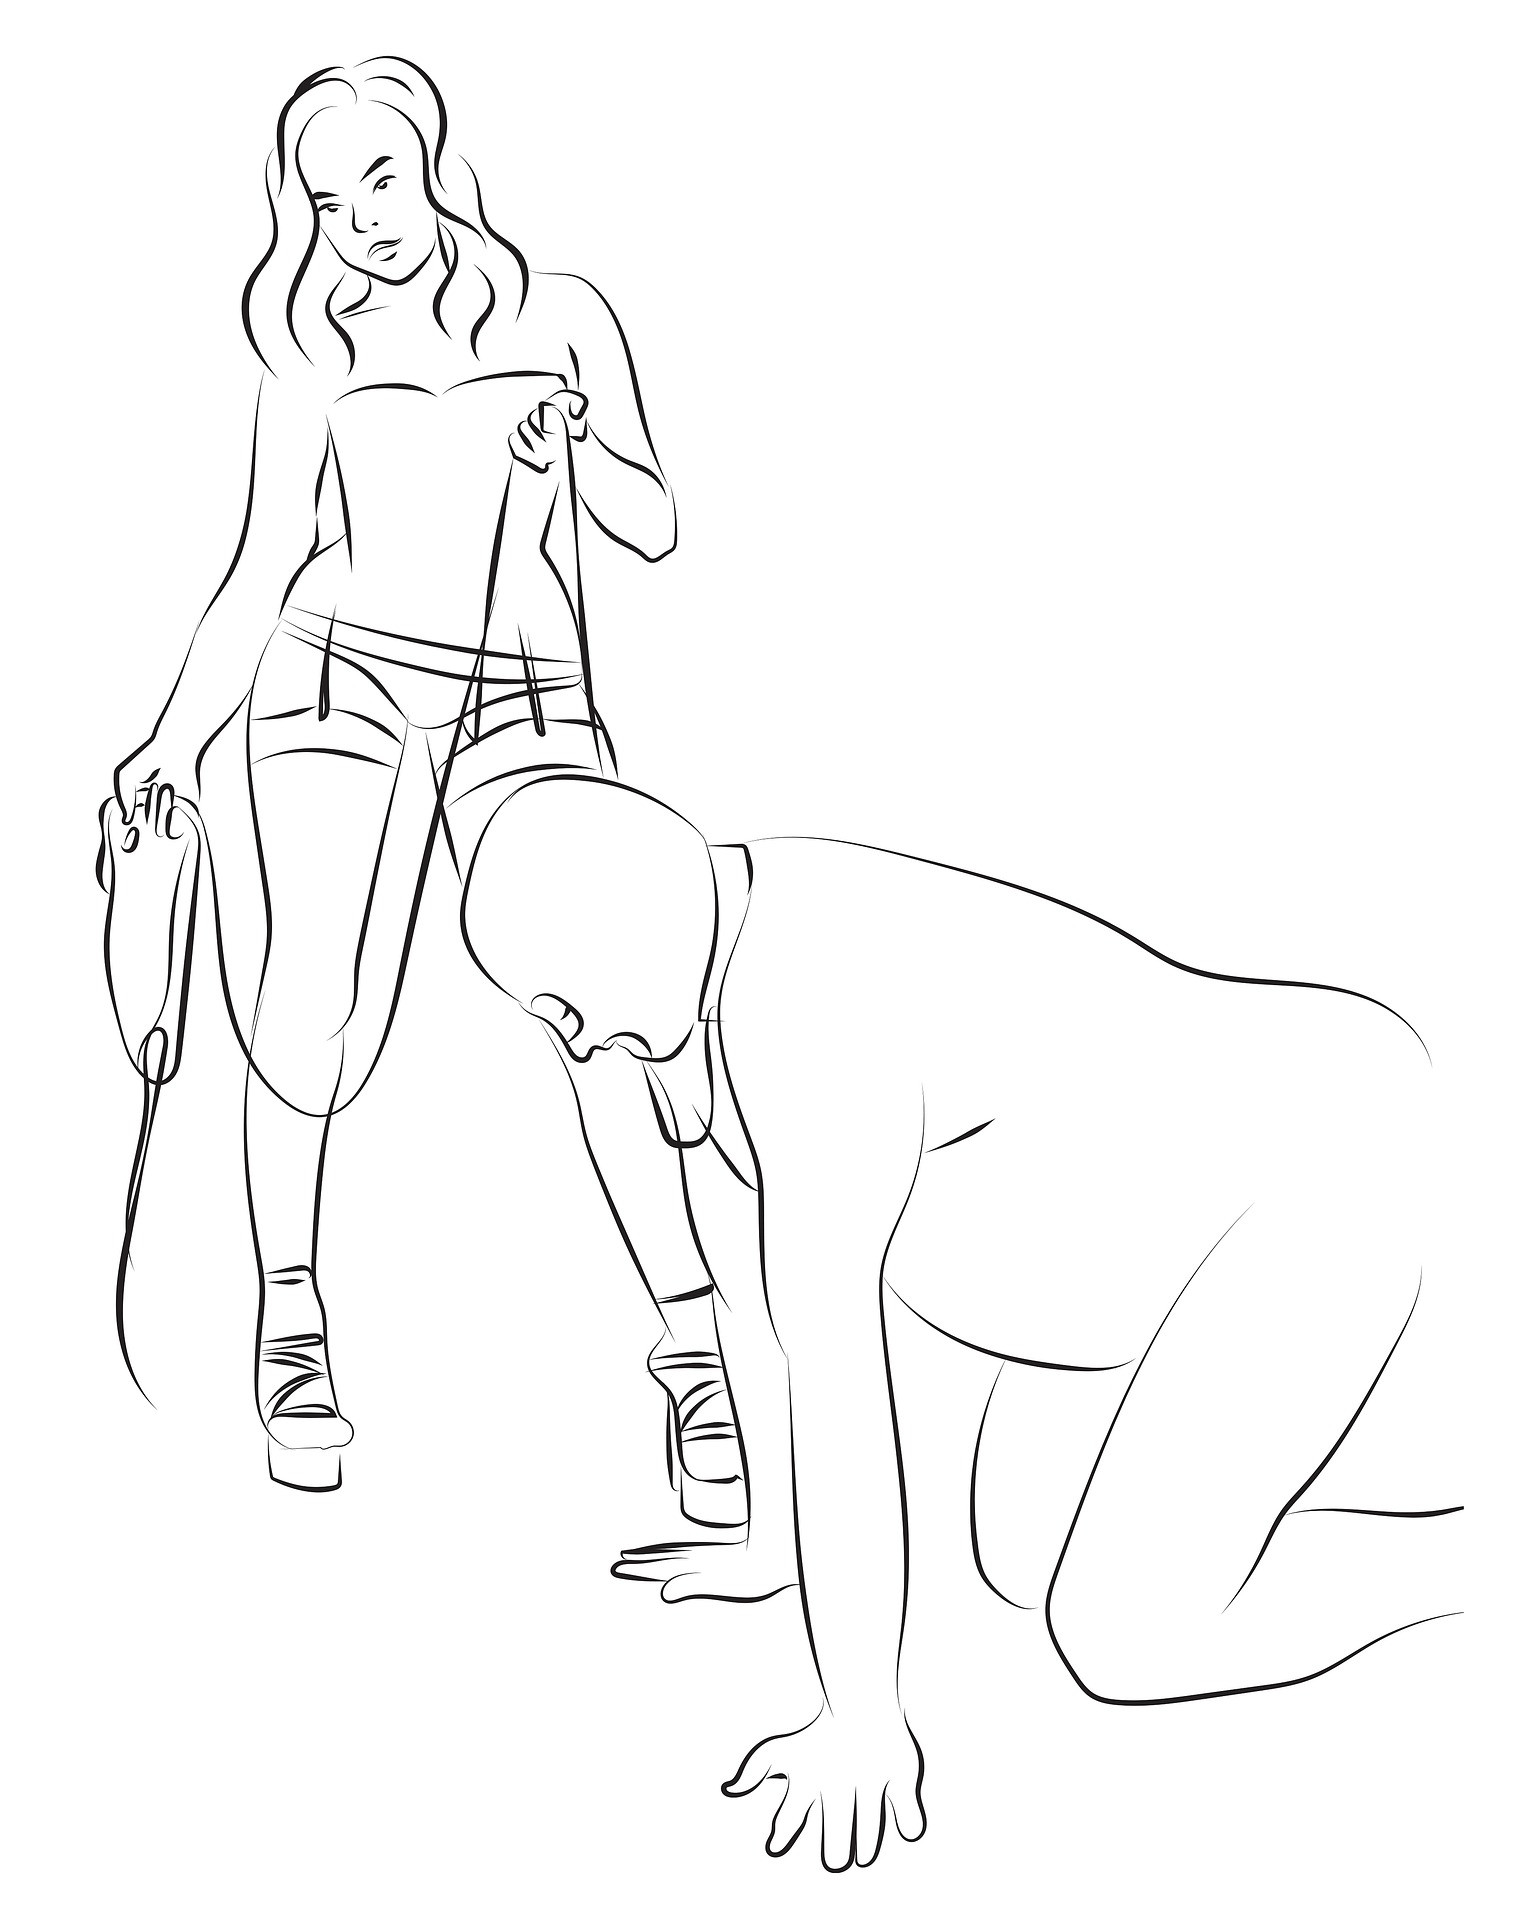
\includegraphics[width=0.7\textwidth]{images/brev64.png}
\end{center}


\breakpage